\documentclass[14pt]{beamer}
\useoutertheme[subsection=false]{miniframes}
\setbeamertemplate{navigation symbols}{}

\usepackage[style=authoryear, sorting=none]{biblatex}
\addbibresource{bibliography.bib}

\graphicspath{{./images/}}

%% symbol definitions
\usepackage{mathtools}
\usepackage{amsmath}
\usepackage{amssymb}
\newcommand{\Spec}{\mathrm{Spec}} % spectrum
\newcommand{\dist}{\mathrm{dist}} % distance
\newcommand{\Num}{\mathrm{W}} % numerical range
\newcommand{\eqdef}{\mathrel{\mathop:}=} % 'defined by' symbol


\title{Spectral Pollution}
\author{Alex H. Room}
\date{2024/06/03}

\begin{document}
\begin{frame}
\titlepage
\end{frame}

\section{Introduction}
\begin{frame}{What are we doing?}
  \centering
  Approximating via finite $T_n \rightarrow T$

  In our case:
  $$(T_n)_{i,j} = (T \varphi_i, \varphi_j)$$
  for a sequence of subsets of an ONB $\{\varphi_i\}_{i \in X_n}$
  \end{frame}

\begin{frame}{Why approximate spectra?}
  \begin{itemize}
    \item Exact calculation is hard! (\textcite{arveson1993role})
    \item No exact methods for:
      \begin{itemize}
        \item (quasi-)Crystallography\footnote{\textcite{colbrook2019how}, \textcite{cances2012periodic}}
        \item Quantum physics\footnote{\textcite{pryce1993numerical}, \textcite{lewin2010spectral}}
        \item Dynamical systems\footnote{\textcite{servadio2022koopman}, \textcite{manning2008descriptor}}
      \end{itemize}
  \end{itemize}
\end{frame}

\begin{frame}{Electronic states (\textcite{pryce1993numerical})}
  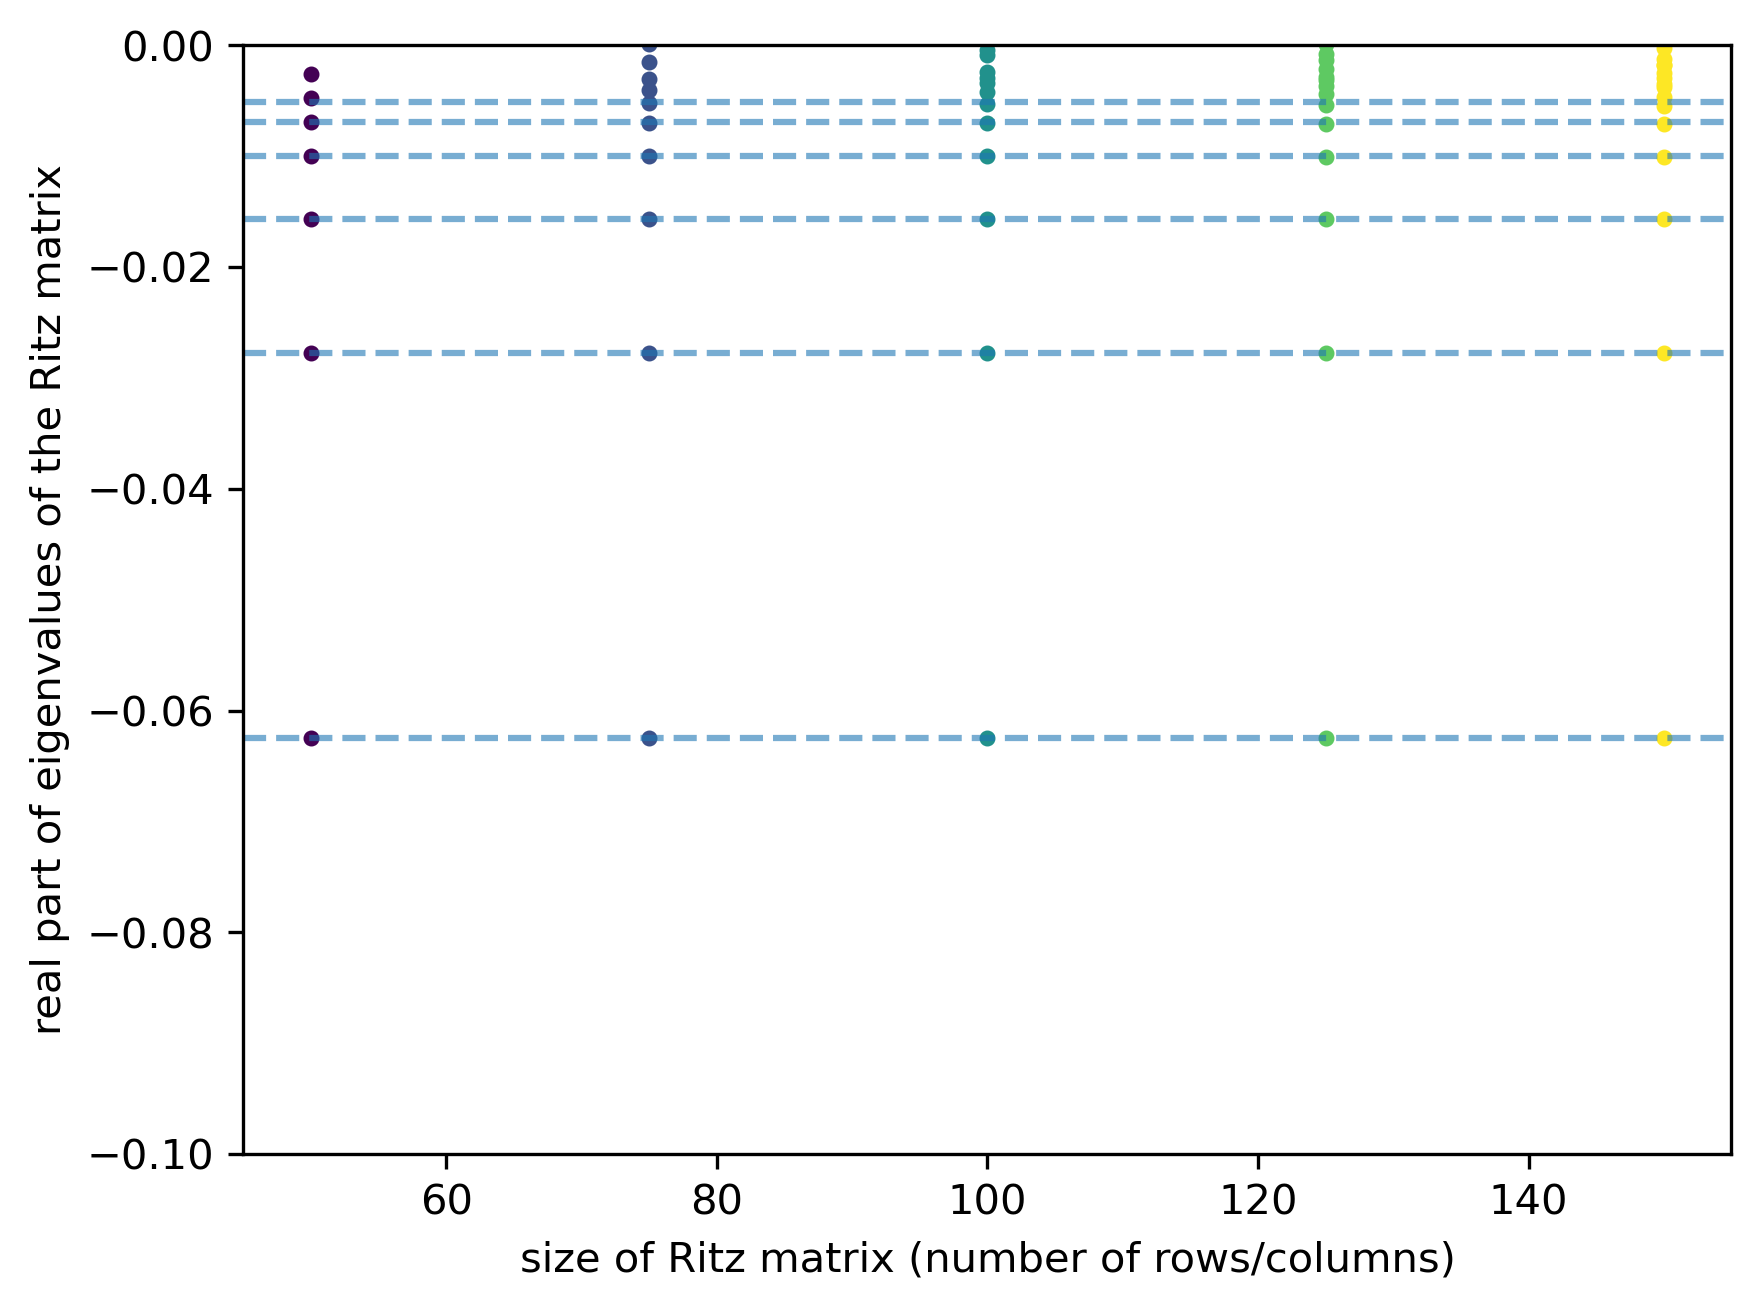
\includegraphics[width=0.9\textwidth]{hydrogen}
\end{frame}

\begin{frame}{Why use truncation methods?}
  \begin{itemize}
    \item Low on \emph{a priori} assumptions
    \item Reduces to linear algebra
    \item Global rather than iterative/local
  \end{itemize}
\end{frame}

\section{Pollution}
\begin{frame}{Numerical methods wishlist}
  We want spectral inclusivity:
  $$\dist(\lambda, \Spec(T_n)) < \varepsilon \quad \forall \lambda \in \Spec(T)$$
  And spectral exactness:
  $$\dist(\lambda_n, \Spec(T)) < \varepsilon \quad \forall \lambda_n \in \Spec(T_n)$$
  Sometimes we can only choose one! (\textcite{colbrook2019how})
\end{frame}

\begin{frame}{What is pollution?}
  \centering
  Consider a sequence $\lambda_n \in \Spec(T_n)$

  such that
  $$\lambda_n \rightarrow \lambda \notin \Spec(T)$$
\end{frame}

\begin{frame}{Example: multiplication operator}
  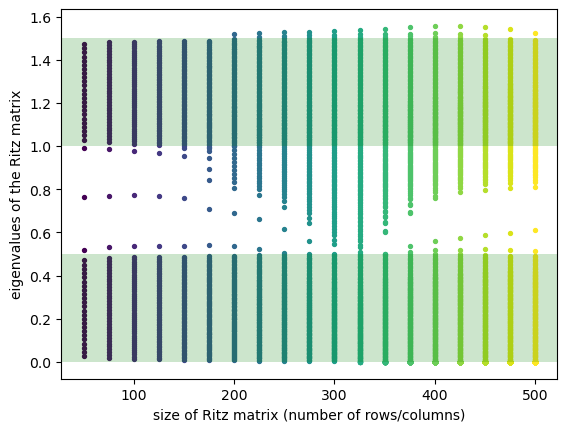
\includegraphics[width=0.9\textwidth]{mult-op-spec}
\end{frame}

\begin{frame}{Non-example: Floquet-Bloch decomposition}
  \centering
  $\bigcup_{|z|=1} \Spec(J_z) = \Spec_e(J)$ 
  \tiny{
    \begin{align*}
      J=
  \begin{pmatrix*}[c]
    \ddots & \ddots & & & \\
    \ddots & b_{-1} & c_0 & & \\
    & a_0 & b_0 & c_1 & \\
    & & a_1 & b_1 & \ddots \\
    & & & \ddots & \ddots \\
  \end{pmatrix*}.
    \leadsto
    J_z = 
    \begin{pmatrix*}[c]
      b_1 & c_2 & & & a_1/z\\
      a_2 & b_2 & c_3 & & & \\
      & a_3 & b_3 & \ddots & & \\
      & & \ddots & \ddots & c_N & \\
      c_{N+1} z & & & a_N & b_N\\
    \end{pmatrix*}.
    \end{align*}
  }
\end{frame}

\begin{frame}{Non-example: almost Mathieu operator}
  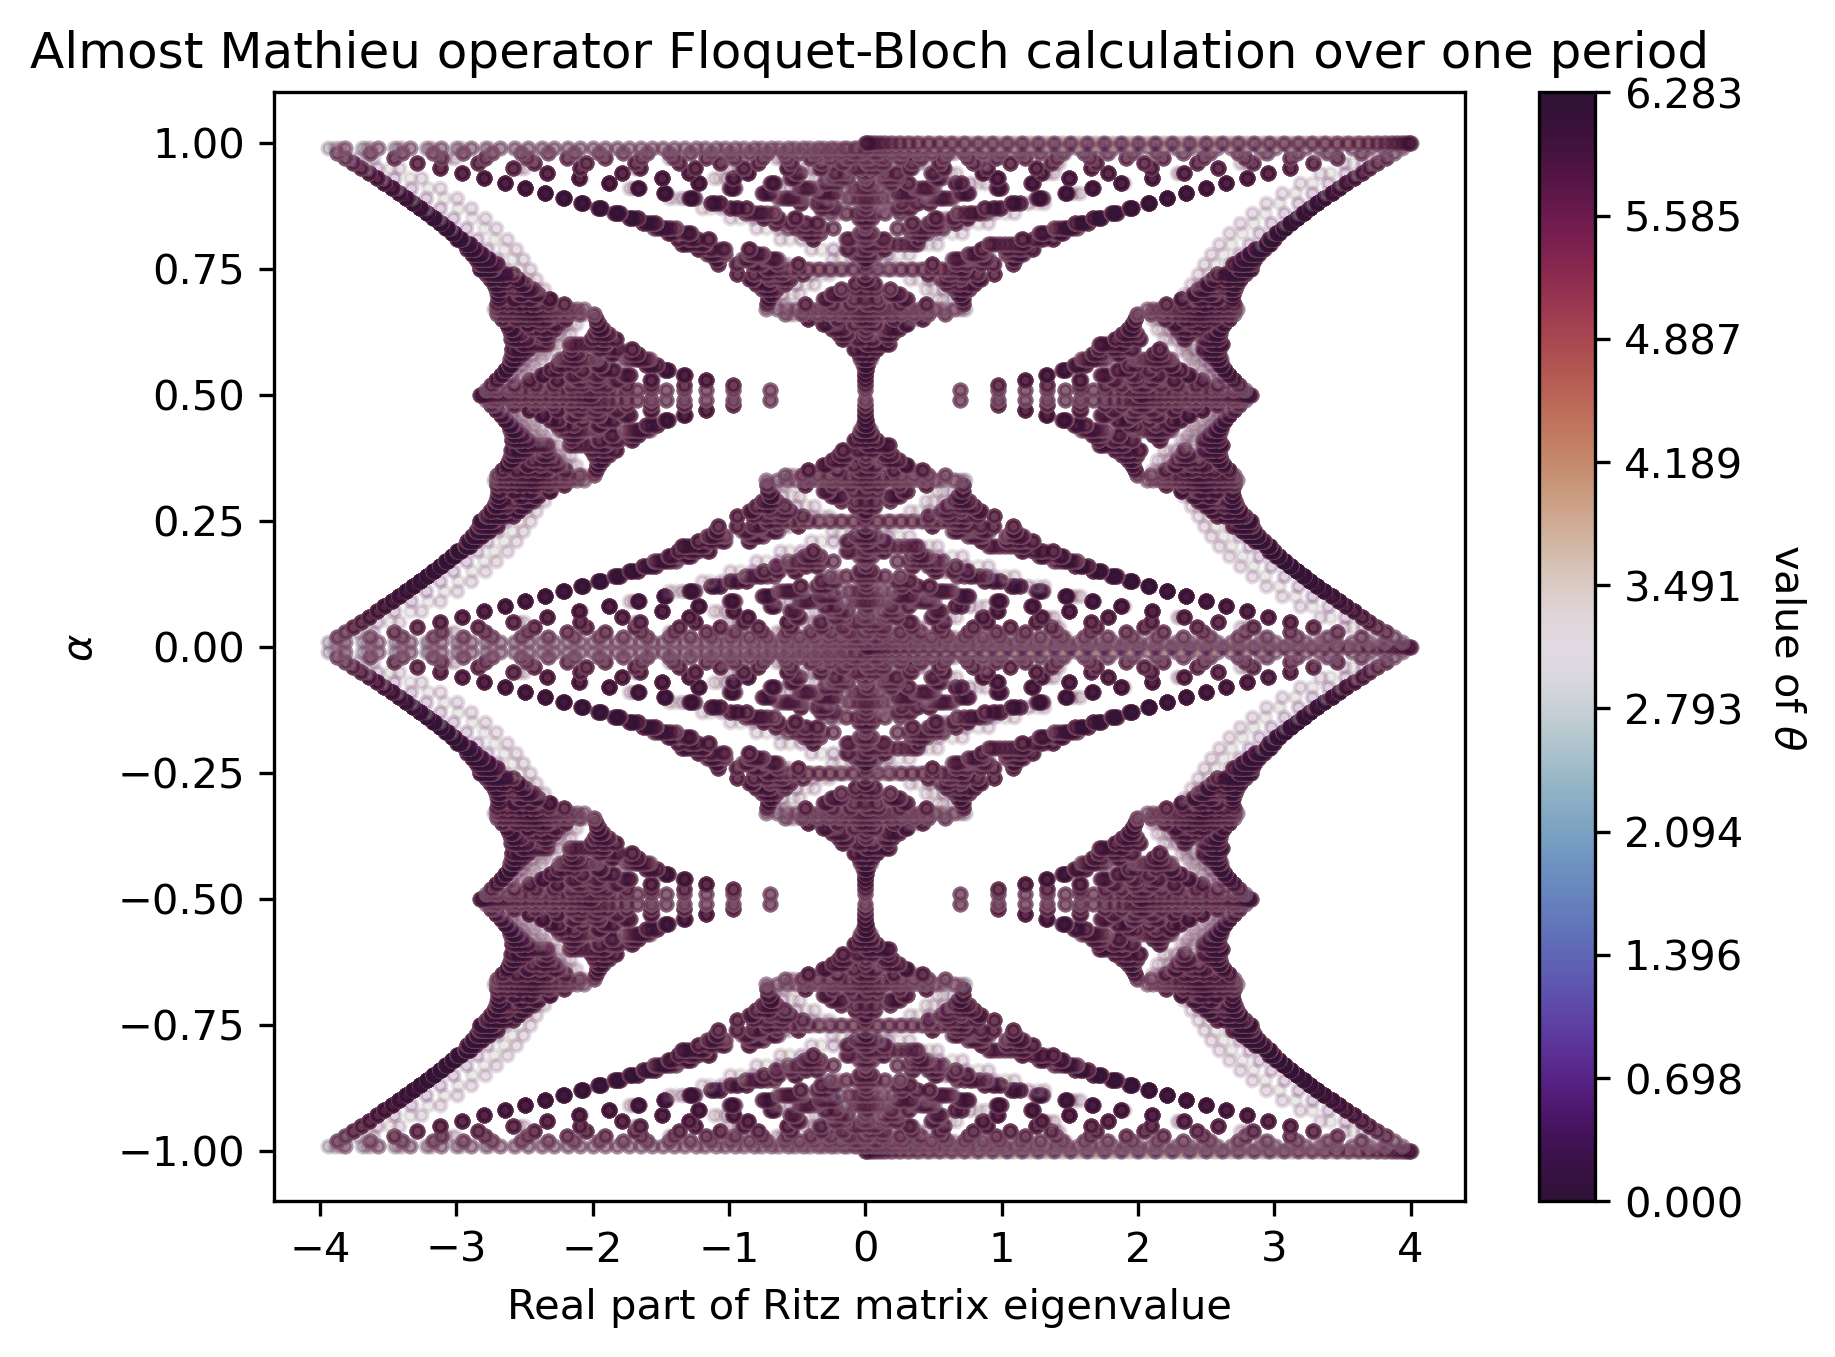
\includegraphics[width=0.9\textwidth]{hofstadter-butterfly}
\end{frame}

\section{Bounding pollution}
\begin{frame}{Numerical range}
  \centering
  $$\Num(T) \eqdef \{(Tu, u) : \|u\| = 1\}$$
  A convex 'sketch' of $T$!
\end{frame}

\begin{frame}{Properties of the numerical range}
  \begin{itemize}
    \item $\Num(T)$ is convex 
    \item $\Spec(T) \subseteq \Num(T)$ if $T$ is normal
    \item From these we can derive classic spectral properties (e.g. self-adjoint $T$ has real spectrum)
    \item[!] $\Num(PTP) \subseteq \Num(T)$ for any truncation $PTP$
  \end{itemize}
\end{frame}

\begin{frame}{Example (Feinberg-Zee)}
  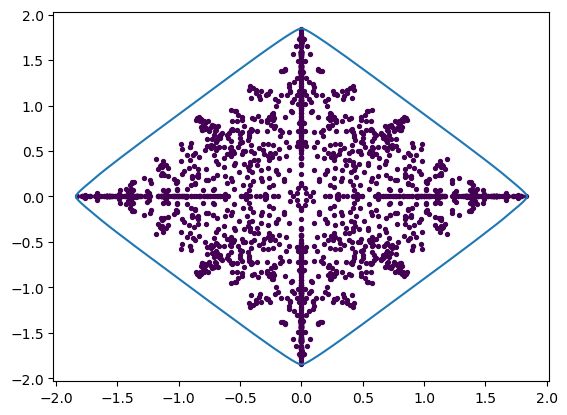
\includegraphics[width=0.9\textwidth]{feinberg-zee-num-range}
\end{frame}

\begin{frame}{Essential spectrum/numerical range}
  \centering
  $$\Num_e(T) = \{\lim_{n \rightarrow 0}(Tu_n, u_n) : \|u_n\| = 1, u_n \rightharpoonup 0\}$$
  \begin{align*}
    \lambda \in \Spec_e(T) \Leftrightarrow \\
    \exists u_n \in \mathcal{H}, \|u_n\|=1 \\
    \|Tu_n - \lambda u_n\| \rightarrow 0 \\
    u_n \rightharpoonup 0
  \end{align*}
\end{frame}

\begin{frame}{Properties of essential spectrum/numerical range}
  \begin{itemize}
    \item $\Num_e(T) \subseteq \overline{\Num(T)}$
    \item $\Spec_e(T) \subseteq \Num_e(T)$
    \item[!] Both invariant under compact perturbations
    \item[!] $\Num_e(T)$ is the smallest set containing all pollution\footnote{\textcite{pokrzywa1979method}, \textcite{bogli2020essential}}
      \begin{itemize}
        \item If $T$ self-adjoint, $\Num_e(T) = \mathrm{conv}\Spec_e(T)$
      \end{itemize}
  \end{itemize}
\end{frame}

\begin{frame}{Pollution-free!}
  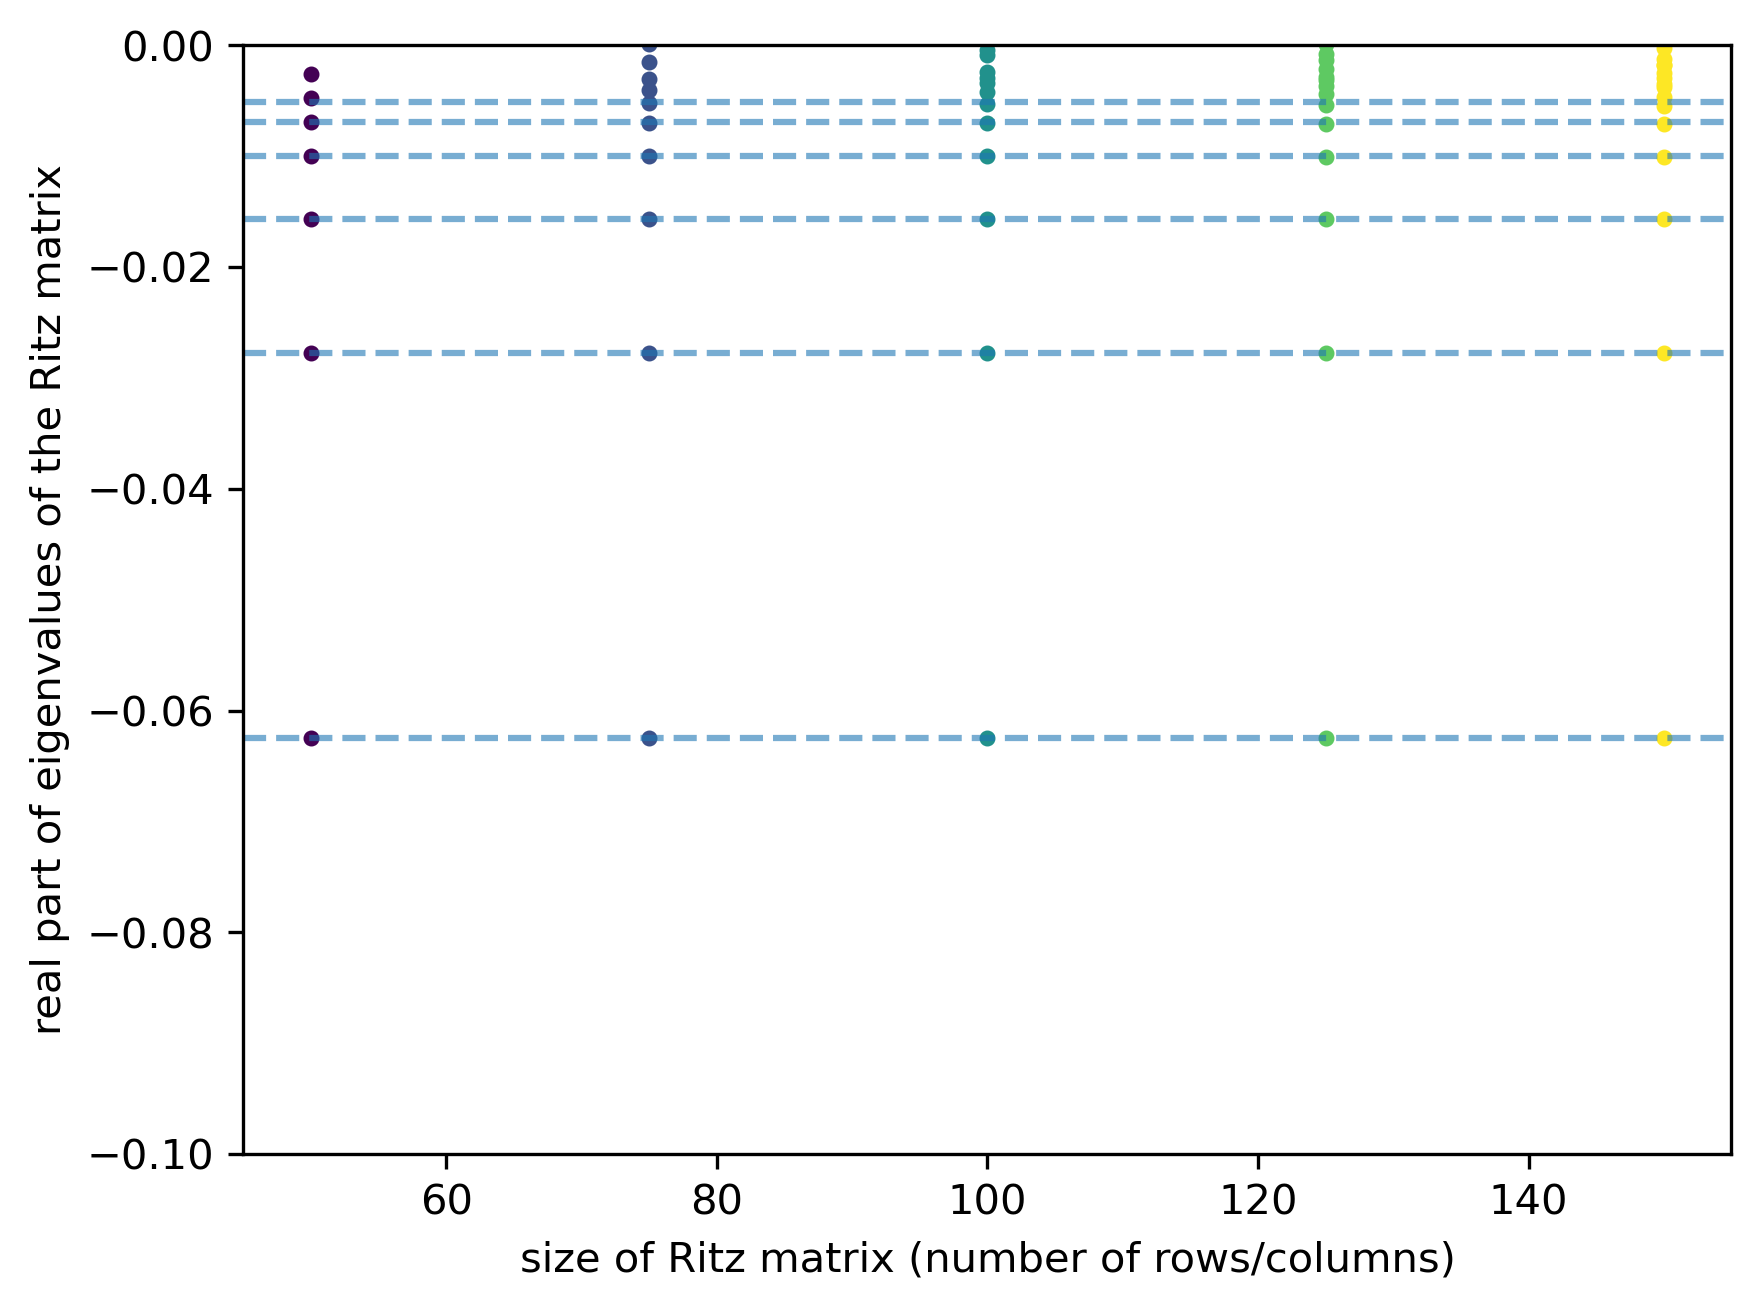
\includegraphics[width=0.9\textwidth]{hydrogen}
\end{frame}

\begin{frame}{Pollution only in the gap}
  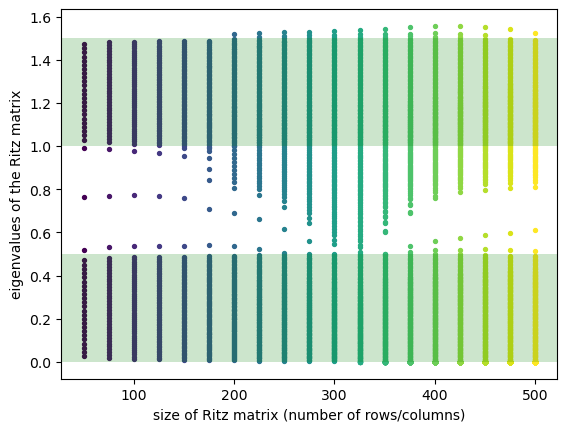
\includegraphics[width=0.9\textwidth]{mult-op-spec}
\end{frame}

\section{Dealing with pollution}
\begin{frame}{Dissipative barrier methods}
  $$\Spec_e(T + iK) = \Spec_e(T)$$
  $$\Num_e(T + iK) = \Num_e(T)$$
  For eigenvector $u$, $Ku \approx u$:
  $$(T + iK)u \approx Tu + iu = (\lambda + i)u$$
\end{frame}

\begin{frame}{Dissipative barrier methods}
  $T_n \leadsto T_n + i\gamma K$: what K? e.g.
  \begin{itemize}
    \item $\mathbf{1}_{[0, R]}$ (\textcite{stepanenko2022spectral})
    \item projection onto $\mathrm{span}\{\varphi_1, ..., \varphi_{n/2}\}$
  \end{itemize}
\end{frame}

\begin{frame}{Example: Sturm-Liouville operator}
  \centering
  $Lu(x) = -\Delta u(x) + (sin(x) - \frac{40}{1+x^2})u(x)$
  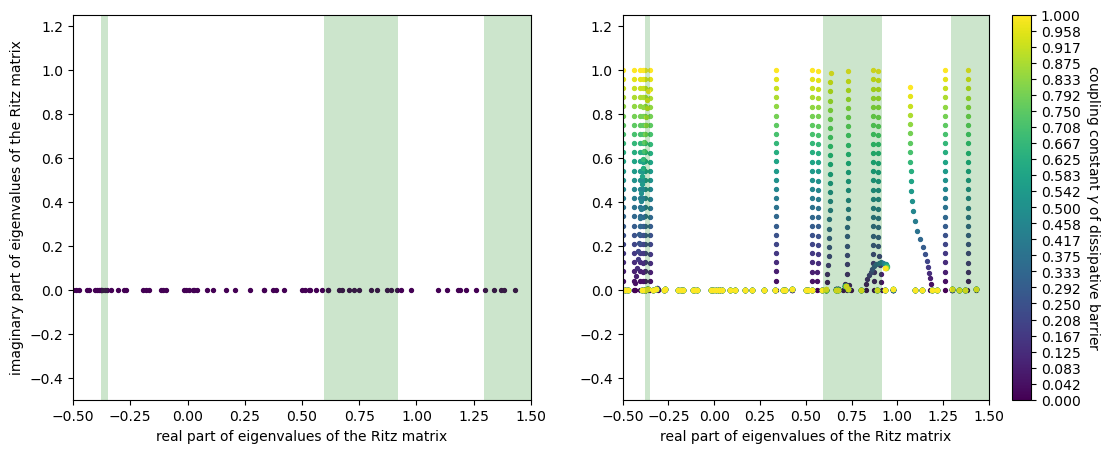
\includegraphics[width=\textwidth]{aceto-coup-presentation}
\end{frame}

\begin{frame}{What else is there?}
  Our moving parts: $T,\mathcal{H}$, \varphi_i
  \begin{itemize}
    \item Auxiliary operator bounds\footnote{\textcite{levitin2002spectral}, \textcite{davies2003spectral}}
    \item Changing boundary conditions or domain\footnote{\textcite{cances2012periodic}, \textcite{aceto2006numerical}}
    \item Good choice of basis\footnote{\textcite{lewin2010spectral}, \textcite{boffi1999problem}}
  \end{itemize}
\end{frame}
\end{document}
